This chapter presents methods to build a visual elevation map and use this map to make the AR.Drone localize itself.
In order to initialize a visual localization and mapping algorithm, a good estimate of the position based on the internal sensors of the AR.Drone is essential.
Section \ref{sec:pose_estimation} describes how the pose is estimated.
When an estimate of the pose is available, a map can be constructed using the method described in Section \ref{sec:mapping}.
Section \ref{sec:localization} describes how this map is used by the AR.Drone to localize itself and reduce the error of the estimated pose.
This localization method is extended in Section \ref{sec:visual-slam-visual-odemetry} to operate as a visual odometry algorithm .
Finally, Section \ref{sec:elevation_map} describes an experimental method to build an elevation map using a single airborne ultrasound sensor.

	\section{Pose estimation}
	\label{sec:pose_estimation}
%In order to initialize a visual localization and mapping algorithm, a good estimate of the position based on the internal sensors of the AR.Drone is essential.
The AR.Drone has several sources of information available about its movements and the majority of its computing power is dedicated to combine these sources into reliable estimates (Section \ref{sec:platform_onboard_intelligence}). In the proposed methods, this information is combined into a state vector, with all information needed to initialize visual localization and mapping.

The AR.Drone is equipped with a number of sensors, which give frequent updates about the motion. 
The inertial sensor measures the body accelerations and angular velocities.
A proprietary filter on board of the AR.Drone converts the angular velocities to an estimated attitude (orientation).
An ultrasound sensor is used to measure the altitude of the vehicle.
In addition to the body accelerations, the AR.Drone sends an estimate of its estimated body velocity (Section \ref{sec:platform_onboard_intelligence}).
This estimate is based on the inertia measurements, aerodynamic model and visual odometry obtained from the relative motion between camera frames.
%Unfortunately, the details of this velocity estimation are
%currently
%not documented by the manufacturer.
The details of this algorithm are proprietary information of the manufacturer. 

The information from the sensors are used in an Extended Kalman Filter (EKF) to estimate the current pose.
An EKF has been considered~\cite{julier2004unscented} the facto standard in the theory of nonlinear state estimation.
The EKF state vector comprises a position vector $p^{W}$, velocity vector $v^{W}$, acceleration vector $a^{W}$ and attitude (orientation) vector $q^{W}$.
All vectors are 3-dimensional Cartesian coordinates.
The position vector $p^{W}$ includes the estimated altitude, which is based on the AR.Drone's ultrasound measurement plus the estimated elevation of the floor (Section \ref{sec:elevation_map}).
An additional altitude vector $h^W$ is added to the EKF state vector, which contains the unmodified ultrasound measurement without the estimated elevation.
Furthermore, it contains first-order and second-order derivatives of the ultrasound measurement.
These derivatives are used by the elevation mapping method (Section \ref{sec:elevation_map}).
%for the elevation mapping method (Section \ref{sec:elevation_map}).
%This vector contains the filtered altitude, first-order and second-order derivatives of the u.

\begin{equation}
x = [ p^{W}  v^{W}  a^{W}  q^{W} h^{W} ]
\label{eq:EKF_state_vecor}
\end{equation}

The sensor data from the AR.Drone is used to fill a measurement matrix.
This measurement matrix is used by the EKF to update the state (Section \ref{sec:background-recursive-state-estimation}).
The attitude (orientation) information from the AR.Drone's proprietary onboard filter is written to the attitude vector of the measurement matrix.
This is possible because the attitude measurements are filtered and debiased onboard of the AR.Drone (Section \ref{sec:platform_onboard_intelligence}).
%The filtered attitude (orientation) from the proprietary onboard filter is written directly to the attitude vector of the EKF's measurement matrix.
%This is possible because 
%Steder et al. \cite{steder2008visual} found that roll and pitch measurements are accurate, even for low-cost sensors and can be directly integrated into the state.
%However, from experiments \ref{Section sec:exp_accel} we found that the low-cost acceleration sensor from the AR.Drone provides unreliable data.
%However, we found that the low-cost acceleration sensor from the AR.Drone provides unreliable data.
%This is modeled by a large uncertainty in the covariance matrix $Q$ of the EKF.
The position of the AR.Drone cannot be estimated directly and is derived from the estimated velocities.
%Unlike the acceleration data, the velocity estimate sent by the AR.Drone is accurate enough for integration into the state.
The velocity estimate sent by the AR.Drone is written to the velocity vector of the measurement matrix.
Based on the previous position $p_{t-1}$, the state's velocity $v_{t}$ and time between measurements $\Delta t$, the new position $p_{t}$ can be calculated as follows:
\begin{equation}
p_{t} = p_{t-1} + v_{t} \times \Delta t + a_{t} \times 0.5 \Delta t^2
\end{equation}
where $\Delta t$ is the variable time (seconds) between the last two measurements.
Instead of using the AR.Drone's onboard velocity estimate, the visual odometry method proposed in Section \ref{sec:visual-slam-visual-odemetry} can be used to determine the AR.Drone's velocity.

In theory, the velocity can be estimated by integrating the body acceleration measurements.
However, the low-cost acceleration sensor from the AR.Drone provides unreliable data, which would result in large velocity errors.
Therefore, the body acceleration measurements are not written to the EKF's measurement matrix.

Similar to the estimated position, the vertical velocity estimate is used to estimate the vehicle's altitude (vertical position).
However, the ultrasound's altitude measurement can be integrated into the EKF's measurement matrix to improve the altitude estimate.
The ultrasound sensor is not sensitive to drift because it provides an absolute altitude measurement.
Relying only on the ultrasound sensor is not optimal since the measurements are affected by the material and structure of the floor (Section \ref{sec:ultrasound_altimeter}).


%\subsection{Inertia measurements}
%\subsection{Onboard filtered measurements}
%\subsection{Vision-based velocity}

	\section{Mapping}
	\label{sec:mapping}
When an estimate of the AR.Drone's pose is available, a map can be constructed to make the AR.Drone localize itself and reduce the error of the estimated pose.
The map consists of a texture map and a feature map.
The texture map is used for human navigation and the feature map is used by the AR.Drone to localize itself.

	\subsection{Visual map}
\label{sec:texture_map}
Now that we have an estimate of the AR.Drone's position and attitude in the world, we can use this information to build a visual map of the environment.
The AR.Drone is equipped with a down-looking camera that has a resolution of $176 \times 144$ pixels.
The frames captured by this camera can be warped on a flat canvas to create a visual map.
Directly merging the frames on the canvas is not possible, because individual frames can be taken from a broad range of angles and altitudes.
Instead, perspective correction is applied and all frames are normalized in size and orientation.

An initial approach of the mapping algorithm was published \cite{Visser2011imav} and presented at the IMAV2011 conference.
This approach uses image stitching \cite{levin2004seamless} to create a visual map.
Knowledge about the AR.Drone estimated state is not used.
%The propagation of stitching errors results in an increasing error.
Because the transformations of all previous frames are used to compute the transformation of the recent frame, the method is sensitive to incorrect transformations.
Therefore, a new mapping method is developped.

Before describing how a frame is warped, some basics about image formation are repeated. %the camera matrix are explained.
The AR.Drone's camera is modeled using a pinhole camera model (Figure \ref{fig:mapping1}).
In this model, a scene view is formed by projecting 3D points into the image plane using a perspective transformation.
%3D camera coordinates are typically described with homogeneous coordinates (Section \ref{sec:background-projective-geometry}).

\begin{figure}[htb]
\centering
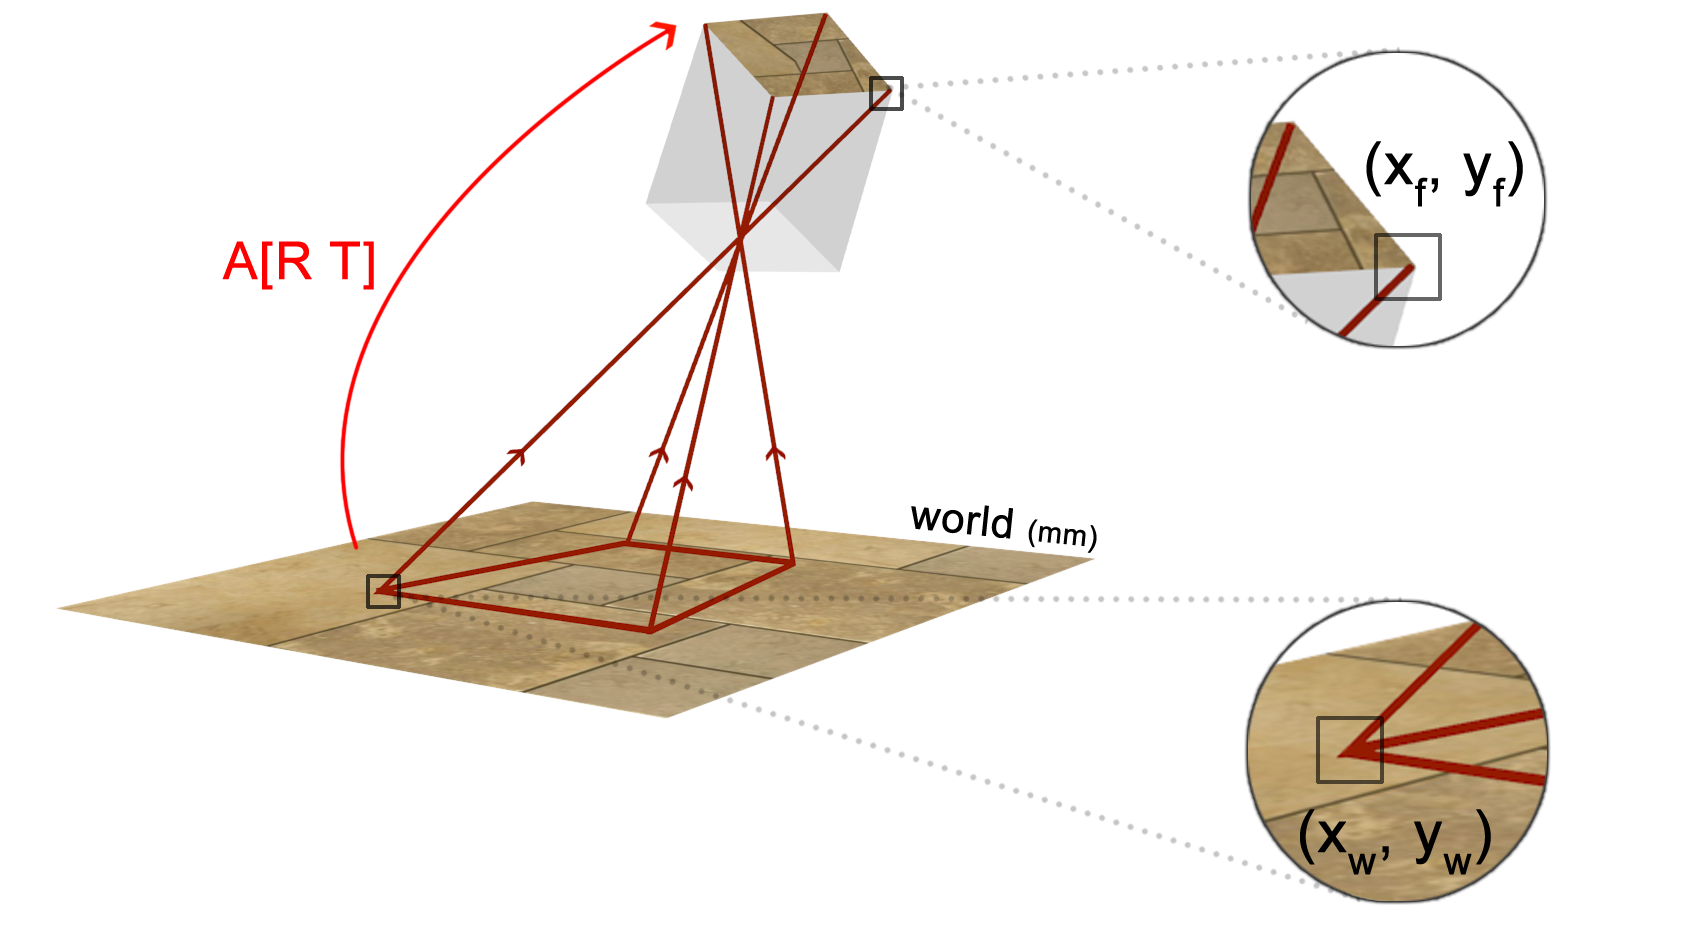
\includegraphics[width=10cm]{images/mapping0.png}
\caption{In the pinhole camera model, a scene view is formed by projecting 3D points into the image plane using a perspective transformation.}
\label{fig:mapping1}
\end{figure}

\begin{equation}
\left[ {
\begin{array}{c} x_f \\ y_f \\ 1 \end{array}
} \right]
= A[R|t]
\left[ {
\begin{array}{c} x_w \\ y_w \\ z_w \\ 1 \end{array}
} \right]
\end{equation}
where $x_f$ and $y_f$ represent a 2D point in pixel coordinates and $x_w$, $y_w$ and $z_w$ represent a 3D point in world coordinates.
The $3 \times 3$ \textit{camera intrinsic} matrix $A$ includes the camera's focal length and principal point.
The $3 \times 4$ joint rotation-translation matrix $[R|t]$ includes the \textit{camera extrinsic} parameters, which denote the coordinate system transformations from 3D world coordinates to 3D camera coordinates. Equivalently, the extrinsic parameters define the position of the camera center and the camera's heading (attitude) in world coordinates.

\begin{figure}[htb]
\centering
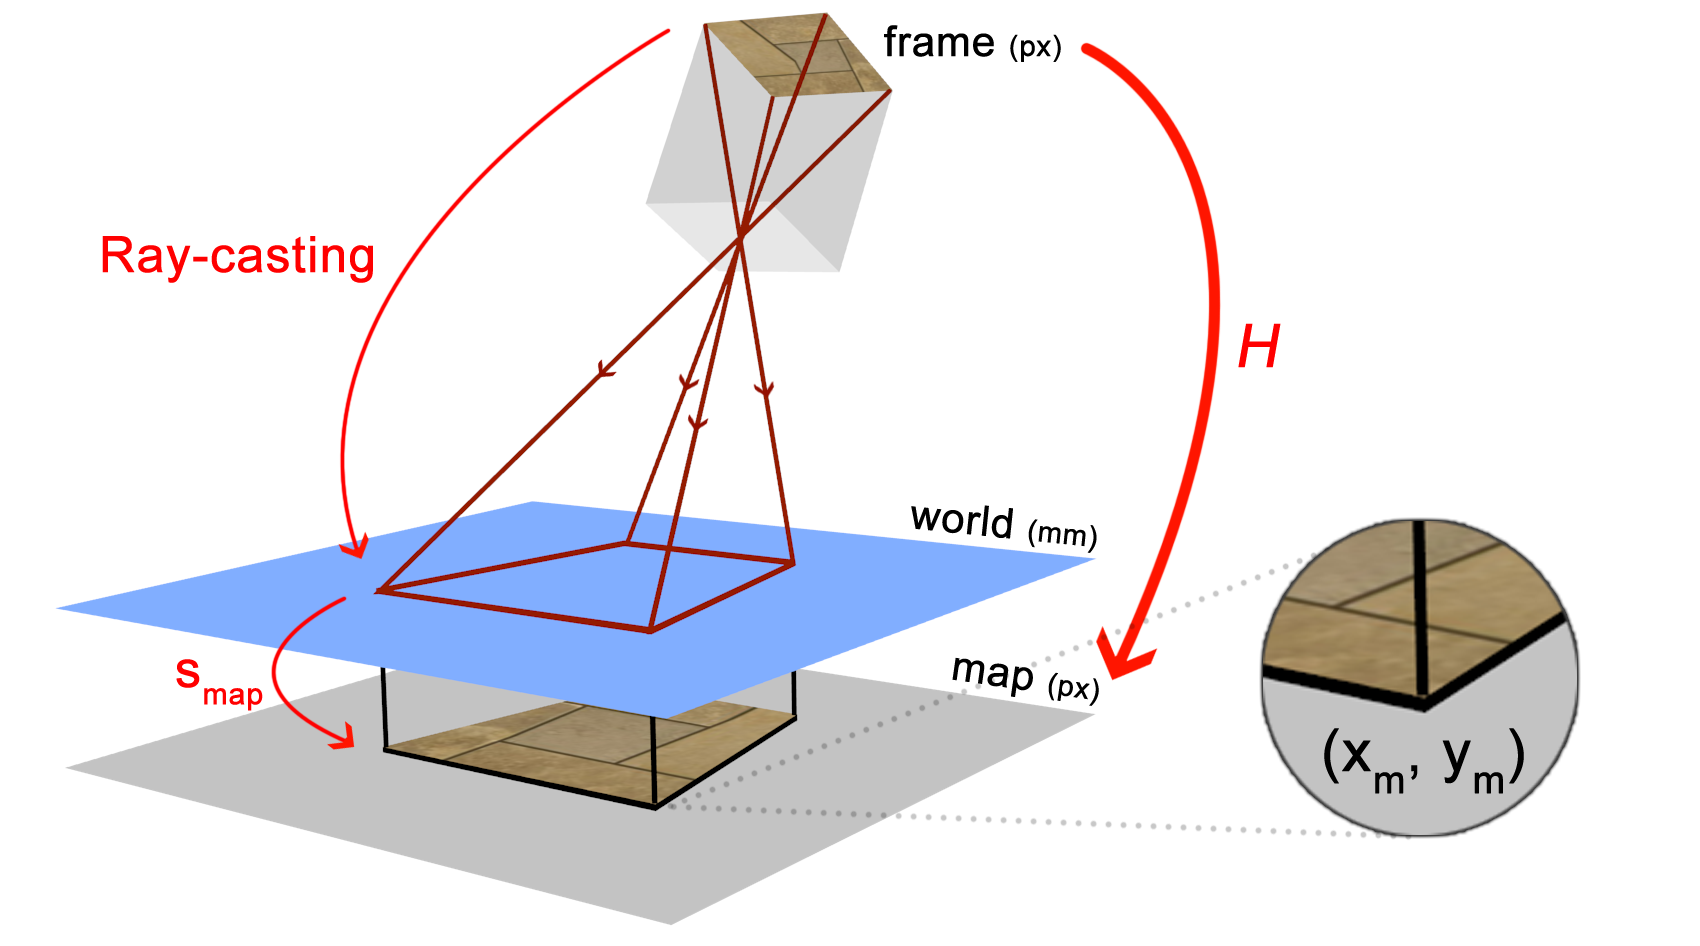
\includegraphics[width=10cm]{images/mapping1.png}
\caption{Visual map: warping a camera frame on the map's canvas. The frame's corners ($\small{px}$) are mapped to 2D world coordinates that lie on the world's plane. The 2D world coordinates of the frame are mapped to the map's canvas coordinates ($\small{px}$). Equation \ref{eq:visual-slam-perspective-transformation} is used to compute the perspective transformation $H$ to transform all pixels of the frame to the corresponding positions on the map's canvas.}
\label{fig:mapping2}
\end{figure}

In order to warp a camera frame on the correct position of the canvas, the algorithm needs to know which area of the world (floor) is captured by the camera.
This is the inverse operation of the image formation described above.
Instead of mapping 3D world coordinates to 2D pixel coordinates, 2D pixel coordinates are mapped to 3D world coordinates ($\small{mm}$).
It is impossible to recover the exact 3D world coordinates, because a pixel coordinate maps to a line instead of a point (i.e., multiple points in 3D world coordinates map to the same 2D pixel coordinate).
\begin{comment}
This is represented in the scaling factor $s$ in the next equation:

\begin{equation}
s \cdot \left[ {
\begin{array}{c} x_w \\ y_w \\ z_w \\ 1 \end{array}
} \right]
= A^{-1}[R|t]
\left[ {
\begin{array}{c} x_f \\ y_f \\ 1 \end{array}
} \right]
\end{equation}
\end{comment}
This ambiguity can be resolved by assuming that all 3D world points lie on a plane ($z_w = 0$), which makes it possible to recover $x_w$ and $y_w$.
The 2D world coordinates of the frame's corners are obtained by casting rays from the four frame's corners (top of Figure \ref{fig:mapping2}).
The 2D world coordinate that corresponds to a frame corner is defined as the point $(x_w,  y_w , 0)$ where the ray intersects the world plane ($z_w = 0$).
Both $x_w$ and $y_w$ are computed as follows:

\begin{equation}
\left[ {
\begin{array}{c} x_w \\ y_w \\ 0 \end{array}
} \right]
 = \frac{(p_0 - l_0) \cdot n}{l \cdot n}
\end{equation}
where $n = \left[ {  \begin{array}{l l l} 0 & 0 & -1 \end{array}  } \right]^T$ is a normal vector to the world plane and $p_0 = \left[ {  \begin{array}{l l l} 0 & 0 & 0 \end{array}  } \right]^T$ is a point on the world plane.
$l$ is a vector in the direction of the ray and $l_0 = p^W$ is a point where the ray intersects the camera plane.
$l$ is computed as follows:

\begin{equation}
l = 
\left|
R
A^{-1}
\left[ {
\begin{array}{c} x_f \\ y_f \\ 1 \end{array}
} \right]
\right|
\end{equation}

Both the camera's extrinsic and intrinsic parameters are required for this operation.
The extrinsic parameters (position and attitude of the camera) are provided by the EKF state vector.
The camera intrinsic parameters are estimated using OpenCV's camera calibration tool\footnote{\url{http://opencv.itseez.com/modules/calib3d/doc/camera_calibration_and_3d_reconstruction.html}}. The implementation is based on the work from \cite{Zhang2000, Bouguet1999}.

%\footnotetext[3]{\url{http://opencv.itseez.com/modules/calib3d/doc/camera_calibration_and_3d_reconstruction.html}}

Now, a relation between the pixel coordinates and world coordinates is known.
However, the 2D world coordinates ($\small{mm}$) need to be mapped to the corresponding 2D pixel coordinates $(x_m, y_m)$ of the map's canvas.
%In the next phase, each frame corner in 2D world coordinates is mapped to the corresponding 2D position on the map's canvas.
A canvas with a fixed resolution of $4.883\small{mm/px}$ is used.
%This means that 1 pixel on the map's canvas corresponds to $4.883\small{mm}$ in world coordinates.

\begin{equation}
\left[ {
\begin{array}{c} x_{m} \\ y_{m} \end{array}
} \right]
= s_{map} \cdot
\left[ {
\begin{array}{c} x_{w} \\ y_{w} \end{array}
} \right]
\end{equation}
where $s_{map} = 1 / 4.884$.

Now, the map's pixel coordinates of the frame corners are known (bottom of Figure \ref{fig:mapping2}).
In order to transform a frame to the map's canvas, a relation between the frame's pixels and map's pixels is required.
A transformation from the frame's corner pixel coordinates and the corresponding pixel coordinates of the map's canvas can be expressed as:

\begin{equation}
\label{eq:visual-slam-perspective-transformation}
\left[ {
\begin{array}{c} x_{m,i} \\ y_{m,i} \\ 1 \end{array}
} \right]
\sim
H
\left[ {
\begin{array}{c} x_{f,i} \\ y_{f,i} \\ 1 \end{array}
} \right]
\end{equation}
The local perspective transformation $H$ is calculated by minimizing the back-projection using a least-squares algorithm.
OpenCV's \textit{findHomography}\footnotemark[3] is used to solve the perspective transformation $H$.
This transformation describes how each frame's pixel needs to be transformed in order to map to the \mbox{corresponding} (sub) pixel of the map's canvas.
The transformation is used to warp the frame on the map's canvas.
By warping the frame on a flat canvas, implicit perspective correction is applied to the frames.
OpenCV's \textit{warpPerspective}\footnote{\url{http://opencv.itseez.com/modules/imgproc/doc/geometric_transformations.html}} is used to warp the frame on the map's canvas.

In this way a texture map can be built. This map consists of a set overlapping textures. The placement and discontinuities of the overlapping textures could be further optimized by map stitching, as described in \cite{Visser2011imav}. Here the texture map is used for human navigation.
For
%automatic navigation
localization a feature map is used, as described in the next section.

			%\subsubsection{Map stitching}
			%\subsubsection{Pose-based mapping}
			%\subsubsection{Optimizing the map}


		\subsection{Feature map}
\label{sec:feature_map}
In addition to the visual map described above, a grid of image features (feature map) is created using a method that is presented in this section.
This feature map will be used for localization purposes, as described in Section~\ref{sec:localization}.
The inertia measurements provide frequent position estimates.
%However, drift will increase the inaccuracy over time.
%However, drift will decrease the accuracy over time.
If the AR.Drone is able to relate a video frame to a position inside the feature map, the vehicle is able to correct this drift long enough to build a map 
as large as the indoor arena of the IMAV competition (as described in Section \ref{sec:exp1-imav-circumstances}).

\begin{figure}[htb]
\centering
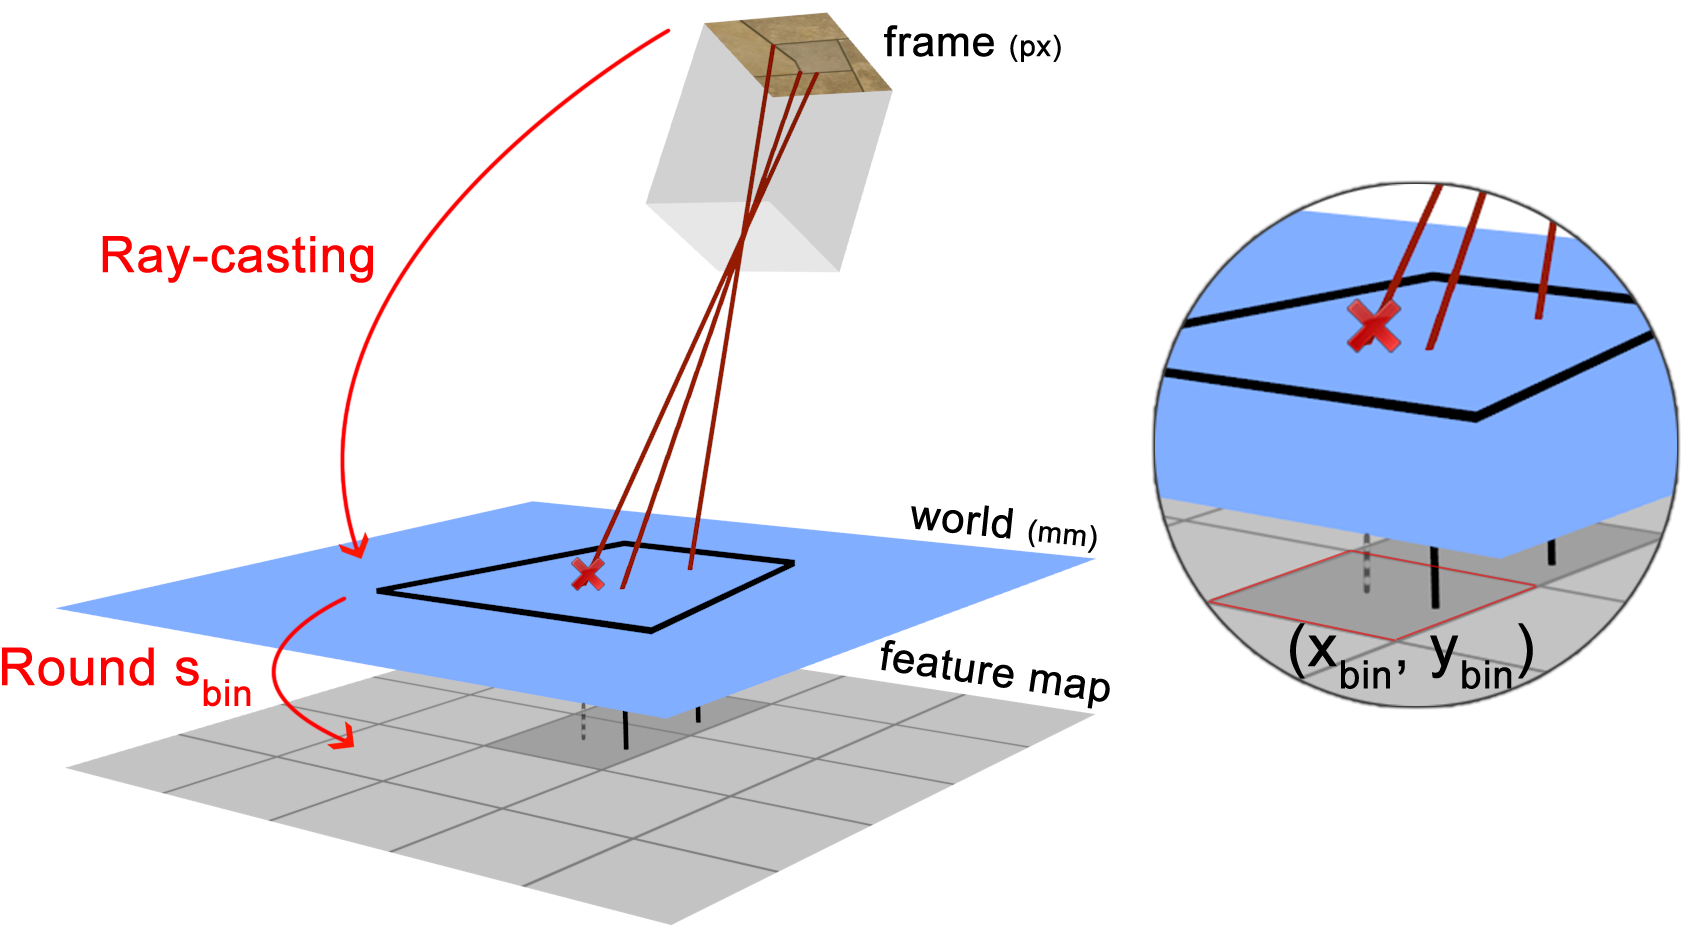
\includegraphics[width=10cm]{images/mapping3.png}
\caption{Feature map: adding visual features to a feature grid. Each feature found in the camera frame is mapped to the corresponding 2D world coordinates. The 2D world coordinates are mapped to the grid cell the feature belongs to. For each cell, only the best feature is stored.}
\label{fig:mapping3}
\end{figure}

A 2D grid with a fixed resolution of $100 \times 100mm$ per cell is used.
%which is nearly equivalent with $20 \times 20\small{px}$.
%Each grid cell corresponds to an area of $100 \times 100\small{mm}$ of the world.
From each camera frame the method extracts Speeded-Up Robust Features (SURF) \cite{Bay2008cviu} that are invariant with respect to rotation and scale.
% SURF features are scale- and rotation-invariant. See Bay2008cviu
Each feature is an abstract description of an interesting part of an image (Section \ref{sec:computer-vision-feature-extraction-matching}).
A SURF feature is described by a center point in image sub-pixel coordinates and a descriptor vector that consists of 64 floats.

Each feature that is detected in a camera frame is mapped to the corresponding cell of the feature map.
A feature's center point ($x_f, y_f$) is transformed to its corresponding position in 2D world coordinates ($x_w, y_w$), visible in the top of Figure \ref{fig:mapping3}.
This is done by casting a ray from the features pixel coordinates in the frame.
The method is similar to the method used for casting ray's from the frame's corners (Section \ref{sec:texture_map}).
Finally, the 2D world position ($x_w, y_w$) of each feature is transformed to the corresponding cell indices ($x_{bin}, y_{bin}$), visible in the bottom of Figure \ref{fig:mapping3}.

\begin{equation}
\left[ {
\begin{array}{c} x_{bin} \\ y_{bin} \end{array}
} \right]
=
Round(
s_{bin}
\cdot
\left[ {
\begin{array}{c} x_{w} \\ y_{w} \end{array}
} \right]
)
\end{equation}
where $s_{bin} = 0.01$.

For each cell, only the best feature (e.g. with the highest response) is kept and the other features are dropped.
%If a cell is already connected to a feature descriptor ($grid_{x,y} \neq \emptyset$), the cell is ignored.
If a cell already contains a feature descriptor ($grid_{x,y} \neq \emptyset$), the cell is ignored.

\begin{equation}
grid_{x,y} = 
\begin{cases}
\arg\max_{d \in D_{x,y}} response(d) & \mbox{if }  grid_{x,y} = \emptyset \\
grid_{x,y}   &   \mbox{else}
\end{cases} 
\end{equation}
where $D_{x,y}$ is the set of features that is mapped to cell $x_{bin} ,y_{bin}$.

%The remaining feature descriptors, including the corresponding world coordinates $x_w, y_w$, are added at the end of a descriptor matrix.
%The indices of these descriptors are written to the corresponding cell of the grid.
%This way, each cell of the grid is connected to a descriptor from the descriptors matrix.
The remaining (best) feature descriptors, including the corresponding world coordinates ($x_w, y_w$), are added to the corresponding grid cells.

%\textbf{TODO: BUFFER}

\begin{comment}
\subsubsection{Processing time}

Processing a single frame and adding it to the map requires approximately $130\small{ms}$ (visual mapping: $20\small{ms}$, feature mapping: $110\small{ms}$).
The AR.Drone's framerate is fixed at 15fps, which is too high to process each single frame in realtime.
In order to achieve realtime mapping, frames that are receiving while another frame is still being process, are dropped.
However, the processing is sufficiently fast to enable seamlessly mapping.
For example, when flying at $1\small{m}$ altitude, the camera (64 degree FOV) perceives $1.24\small{m}$ floor.
The maximum horizontal speed to achieve seamlessly mapping at 15fps is 
% $(1.24 * 15 = 
$18.75\small{m/s}$, which is nearly four times the default maximum speed of the AR.Drone ($5\small{m/s}$).
With reduced framerate (7.7fps instead of 15 fps), the maximum horizontal speed is 
% $1.24 * 7.7 = 
$9.55\small{m/s}$, which is significantly faster than the AR.Drone's default maximum speed.
\end{comment}


	\section{Localization}
\label{sec:localization}

The feature map created in the previous section can be used for absolute position estimates, at the moment of loop-closure (when the AR.Drone observes a location where it has observed before).
This allows to correct the drift that originates from the internal sensors of the AR.Drone.
The
%inertia
sensor measurements provide frequent velocity estimates.
However, the estimated position will drift over time, because the errors of the
%inertia measurements
velocities estimates are being accumulated.
The feature map that is created can be exploited to reduce this drift, because localization against this map provides absolute positions of the vehicle.
These absolute positions are integrated into the EKF and improve the estimated position and reduce the covariance of the state.

When a camera frame is received, SURF features are extracted.
Each feature consists of a center position in pixel coordinates ($x_f, y_f$) and a feature descriptor.
A feature's center point ($x_f, y_f$) is transformed to its corresponding position in 2D world coordinates ($x_w, y_w$), visible in the top of Figure \ref{fig:mapping3}.
This is done by casting a ray from the features pixel coordinates in the frame.
The method is similar to the method used for casting ray's from the frame's corners (Section \ref{sec:texture_map}).

%The pixel coordinates of the features are transformed to 2D world coordinates.
%The method used is already described in Section X.

The next step is matching the feature descriptors from the camera frame against the feature descriptors from the feature map.
When the feature map is quite large, this process becomes slow.
However, the estimated position of the vehicle can be used to select a subset of the feature map.
This can be done by placing a window that is centered at the vehicle's estimated position.
The covariance of the estimated position can be used to determine the size of the window.
The set of frame descriptors (query descriptors $D_q$) is matched against the map descriptors (training descriptors $D_t$).
Matching is done using a brute force matcher that uses the $L^2$ norm as similarity measure.
For each query descriptor $d_q$ from the frame, function $C(d_q)$ selects the training descriptor $d_t$ from the map that minimizes the $L^2$ norm:


\begin{equation}
C(d_q) = \arg\min_{d_t \in D_T} L^2(d_q, d_t)
\end{equation}
where $D_T$ is the set of map descriptors within a window around the estimated position.
The $L^2$ distance between two descriptors $a$ and $b$ is defined as:

\begin{equation}
L^2(a,b) =\sqrt { \sum_{i=1}^{N} \left| a_i - b_i \right| ^2 }
\end{equation}
where $N = 64$ is the length of the SURF descriptor vector.

Each query descriptor (frame) is matched against the descriptor from the training descriptors (map) that is most similar.
Please note it is possible that multiple descriptors from the frame are matched against a single descriptor from the map.

For each match $C(d_q, d_t)$ the 2D world coordinates $(x_{w, d_q}, y_{w, d_q})$ and $(x_{w, d_t}, y_{w, d_t})$ of both descriptors are already computed.
These point pairs can be used to calculate a transformation between the query points (frame) and training (map) points.
This transformation describes the relation between the EKF estimated vehicle position (described in Section~\ref{sec:pose_estimation}) and the position according to the feature map.

\begin{figure}[htb]
\centering
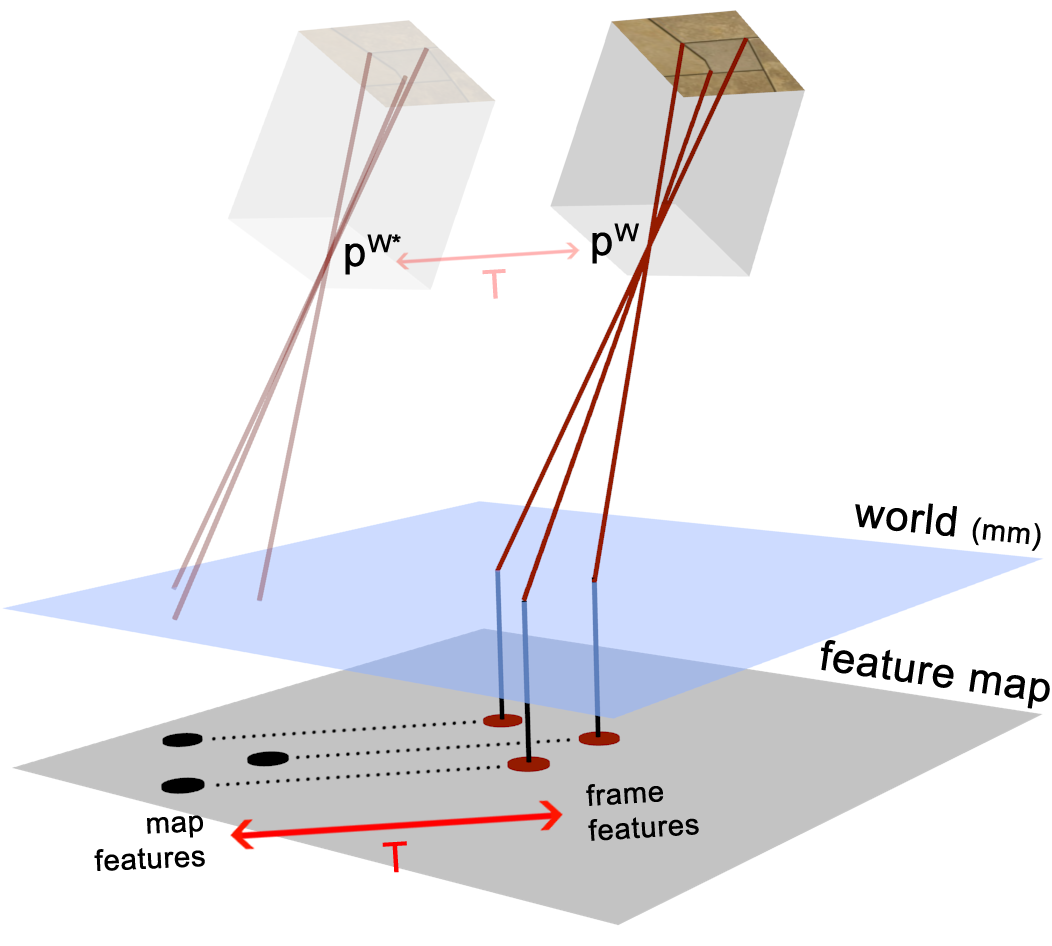
\includegraphics[width=9cm]{images/localization1.png}
\caption{Localization: features from the camera frame (red circles) are matched against the features from the feature map (black circles). All the feature points (pixels) are converted to 2D word coordinates. The translation $T$ between both feature sets is calculated and used to correct the estimated position of the AR.Drone.}
\label{fig:localization1}
\end{figure}

%This localization method allows us to exploit the feature map created in Section~\ref{sec:feature_map} and get absolute position estimates which can be used to %autonomously navigate the AR.Drone, as demonstrated in the next section.






\subsection{Pose recovery approaches}
\label{sec:pose-recovery}
Different types of transformations can be used to describe the relation between the point pairs (e.g., perspective transformation or affine transformation).
However, if not all of the point pairs fit the transformation (due to outliers), the initial transformation estimate will be poor.
Random Sample Consensus (RANSAC) \cite{fischler1981random} is used to filter the set of matches in order to detect and eliminate erroneous matches (point pairs).
RANSAC tries different random subsets of corresponding point pairs.
It estimates the transformation using this subset and then computes the quality of the computed transformation by counting the number of inliers.

Since the point pairs are normalized,
%,(i.e., all pixel coordinates are transformed to 2D world coordinates),
the perspective deformation and scale differences between the point pairs (matches) are already removed.
The remaining degrees of freedom are the translation and rotation between the point pairs. 
Perspective transformation and affine transformation provide more degrees of freedom than required.
This is potentially dangerous, because an incorrect transformation may still result in a high percentage of inliers.
For example, this may happen when multiple query descriptors (from the frame) are matched against a single training descriptor (from the map).
In that case, a perspective or affine transformation is found that scales all points to a single position.
This transformation does not correspond with the actual translation and rotation, but is a valid transformation according to the RANSAC algorithm.

Instead of computing a full perspective, affine or Euclidean transformation, a more pragmatic approach is used.
Here, only the translation in $x$ and $y$ direction is estimated.
The best translation is chosen with a modified RANSAC algorithm, which uses covariance between matches instead of the number inliers as quality measure.
The rotation is estimated independently, as described at the end of this section.

A translation hypothesis $T$ is computed by taking a subset of three random point pairs and calculating the mean translation:

\begin{comment}
$M_{train} = \begin{pmatrix}
x_{0,t,w} & y_{0,t,w}
\\
x_{1,t,w} & y_{1,t,w}
\\
x_{2,t,w} & y_{2,t,w}
\end{pmatrix}$

$M_{query} = \begin{pmatrix}
x_{0,q,w} & y_{0,q,w}
\\
x_{1,q,w} & y_{1,q,w}
\\
x_{2,q,w} & y_{2,q,w}
\end{pmatrix}$

\begin{equation}
T = (M_{train} - M_{query}) / N
\end{equation}


\begin{equation}
T =
\left[ {
\begin{array}{c}
 \frac{\sum_{i}^{N} (x_{t,w} - x_{q,w})}{N}
\\
 \frac{\sum_{i}^{N} (y_{t,w} - y_{q,w})}{N}
\end{array}
} \right]
\end{equation}


\end{comment}


\begin{equation}
T_x = \frac{\sum_{i}^{N} (x_{w, d_t, i} - x_{w, d_q, i})}{N}
\end{equation}
\begin{equation}
T_y = \frac{\sum_{i}^{N} (y_{w, d_t ,i} - y_{w, d_q, i})}{N}
\end{equation}
where $N = 3$ is the number of point pairs.
The standard deviation of translation  $T$ is defined as:
\begin{equation}
\sigma_x = \sqrt{  \sum_{i}^{N}   ((x_{w, d_t} - x_{w, d_q}) - T_x)^{2}   }
\end{equation}
\begin{equation}
\sigma_y = \sqrt{  \sum_{i}^{N}   ((y_{w, d_t} - y_{w, d_q}) - T_y)^{2}   }
\end{equation}
The confidence $c$ of translation $T$ is computed using the standard deviation:
\begin{equation}
c_{T} = 1 -   \sigma_x / \theta_{d} -  \sigma_y / \theta_{d}
\end{equation}
where $\theta_d$ = 200.
Similar to RANSAC, this step is repeated $k$ times to test multiple hypotheses.
After all repetitions are performed, the translation with highest confidence $T_{best}$ is used as final translation.

The advantages of this approach are threefold.
By using the confidence, instead of the number of inliers (as mostly done in classic RANSAC), a more robust estimate of the translation can be made. 
Furthermore, this approach eliminates the additional degrees of freedom that can results in incorrect transformations (as described above).
An additional benefit of the two degrees of freedom approach is its efficiency, allowing a great number of RANSAC iterations to find the optimal subset of point pairs.

If the confidence $c_{T}$ of the translation $T_{best}$ exceeds a threshold, the transformation $T$ is added to the estimated position $p^W$ to compute the corrected position $p^{W*}$. This corrected position is integrated in the EKF as measurement with low covariance.
Please note this method requires that the estimated yaw of the vehicle is close to the actual yaw.
A large difference between estimated and actual yaw results in low confidence $c_T$.
%Localization on regular basis should sufficiently correct errors in the estimated yaw, when using the method described below.
Therefore, the next paragraph describes a method to reduce the error in the estimated yaw.
Performing this optimization on regular basis should sufficiently correct errors in the estimated yaw.


If the confidence is exceptionally high (i.e., good matches are found), the selected point pairs are used to determine the rotation between the estimated yaw and the real yaw of the vehicle. This rotation is used to correct the drift in yaw.
The rotation is computed using Kabsch algorithm \cite{Kabsch:a12999}.
This method computes the optimal rotation matrix that minimizes the RMSD (root mean squared deviation) between two sets of points.
% (in this case the sets that are used to determine the translation).
These sets of points are the same two sets of points used to compute the translation, as described above.
%Like the translation, the rotation is added to the estimated rotation to calculate the correct rotation.
This rotation is added as an offset to all future yaw measurements.
%This rotation is directly written to the EKF state.

In Section \ref{sec:results-pose-recovery}, an experiment is performed to validate that the proposed pose recovery method outperforms three other approaches.



\section{Visual odometry}
\label{sec:visual-slam-visual-odemetry}
The AR.Drone's onboard intelligence estimates the velocity using two complementary visual odometry algorithms and an aerodynamic model of the AR.Drone.
However, its limited processing power requires the use of lightweight features and algorithms, which may affect the accuracy of the estimated velocities.
Running a visual odometry algorithm offboard relaxes the computational limitations, allowing more complex (better) features and algorithms.
In this section, the localization method presented in the previous section is modified to operate as a visual odometry algorithm.
Instead of matching the last frame against the feature map, now the last frame is matched against the previous frame.
The resulting velocity estimates can be merged with the onboard velocity estimates to improve the accuracy of estimated velocity.

When a camera frame $f_t$ is received, SURF features are extracted.
Each feature consists of a center position in pixel coordinates ($x_f, y_f$) and a feature descriptor.
A feature's center point ($x_f, y_f$) is transformed to its corresponding position in 2D world coordinates ($x_w, y_w$).
This is done using ray-casting, as described in Section \ref{sec:texture_map}.
Contrary to the previous sections, the origin of the ray is set to $(0, 0, z)$, such that the estimated position of the AR.Drone doesn't influence the visual odometry calculations.
% where the position of the AR.Drone is set to $(0, 0)$.

The next step is matching the feature descriptors from the last frame $f_t$ against the feature descriptors from the previous frame $f_{t-1}$.
The set of descriptors $D_{t}$ from the current frame $f_t$ is matched against the descriptors $D_{t-1}$ from the previous frame $f_{t-1}$.
Matching is done using a brute force matcher that uses the $L^2$ norm as similarity measure.
For each descriptor $d_{t}$ from frame $f_t$, function $C(d_{t})$ selects the descriptor $d_{t-1}$ from the previous frame $f_{t-1}$ that minimizes the $L^2$ norm:

\begin{equation}
C(d_{t}) = \arg\min_{d_{t-1} \in D_{t-1}} L^2(d_t, d_{t-1})
\end{equation}
The $L^2$ distance between two descriptors $a$ and $b$ is defined as:

\begin{equation}
L^2(a,b) =\sqrt { \sum_{i=1}^{N} \left| a_i - b_i \right| ^2 }
\end{equation}
where $N = 64$ is the length of the SURF descriptor vector.

\begin{figure}[htb!]
  \begin{center}
    \subfigure[Frame $f_{t-1}$]{\label{visual-slam-visual-odometry1}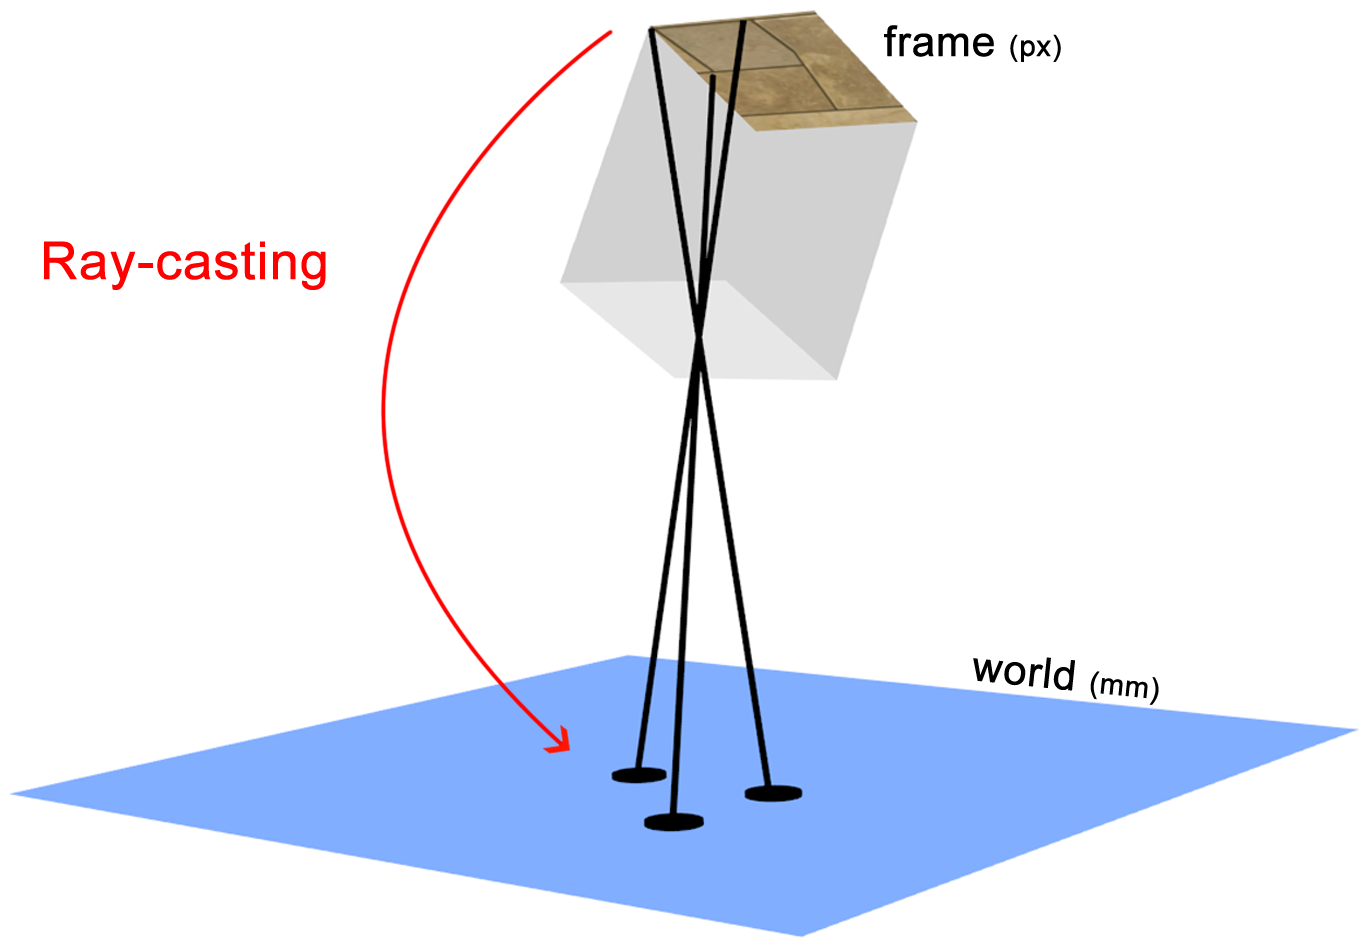
\includegraphics[width=0.33\linewidth]{images/visual_odometry1.png}}
    \subfigure[Frame $f_t$]{\label{visual-slam-visual-odometry2}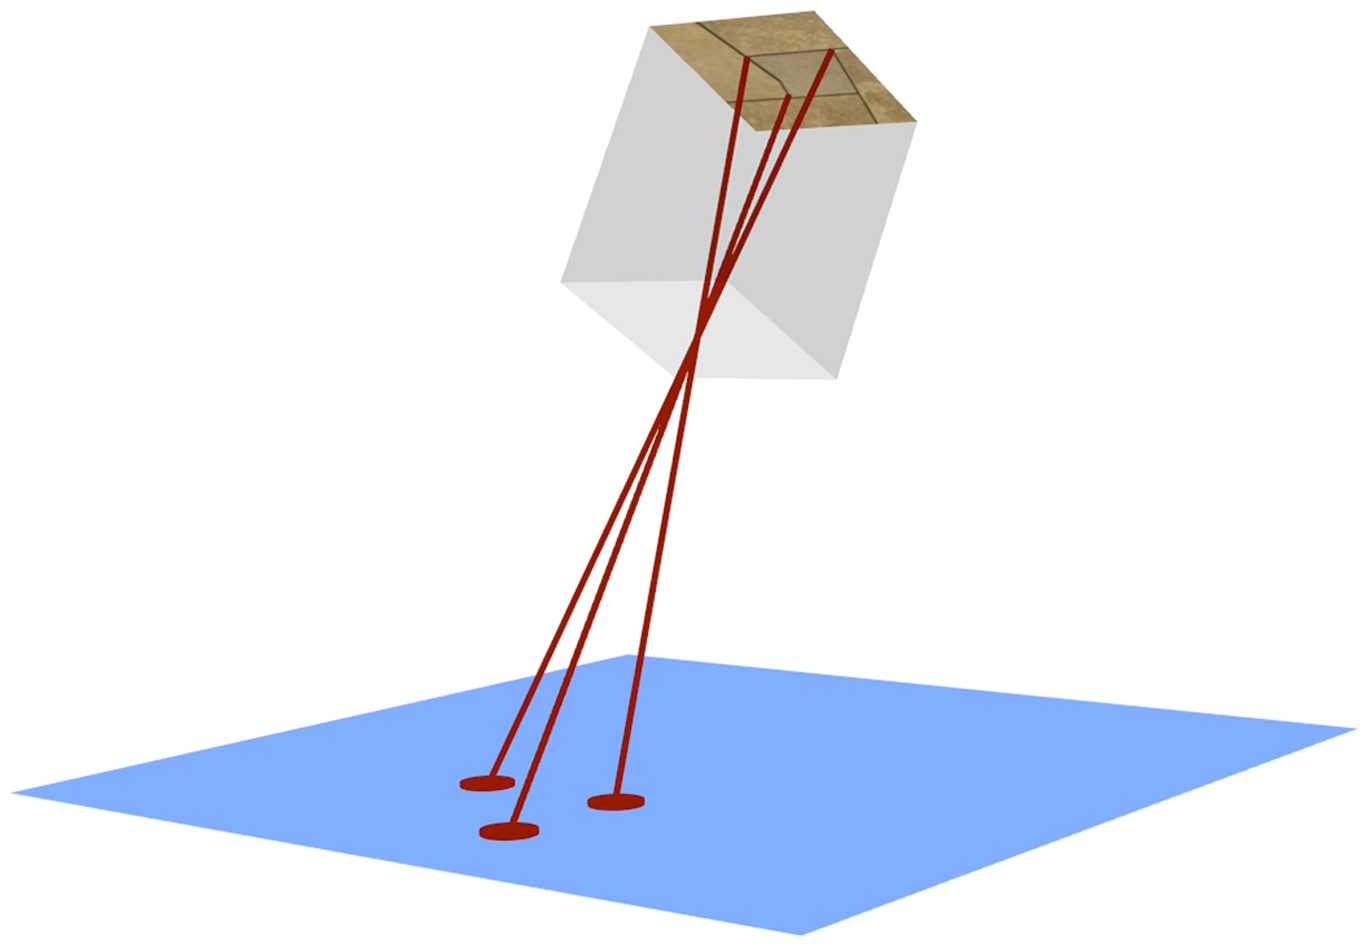
\includegraphics[width=0.33\linewidth]{images/visual_odometry2.png}}
    \subfigure[Feature coordinates of frame $f_{t-1}$ and $f_t$]{\label{visual-slam-visual-odometry3}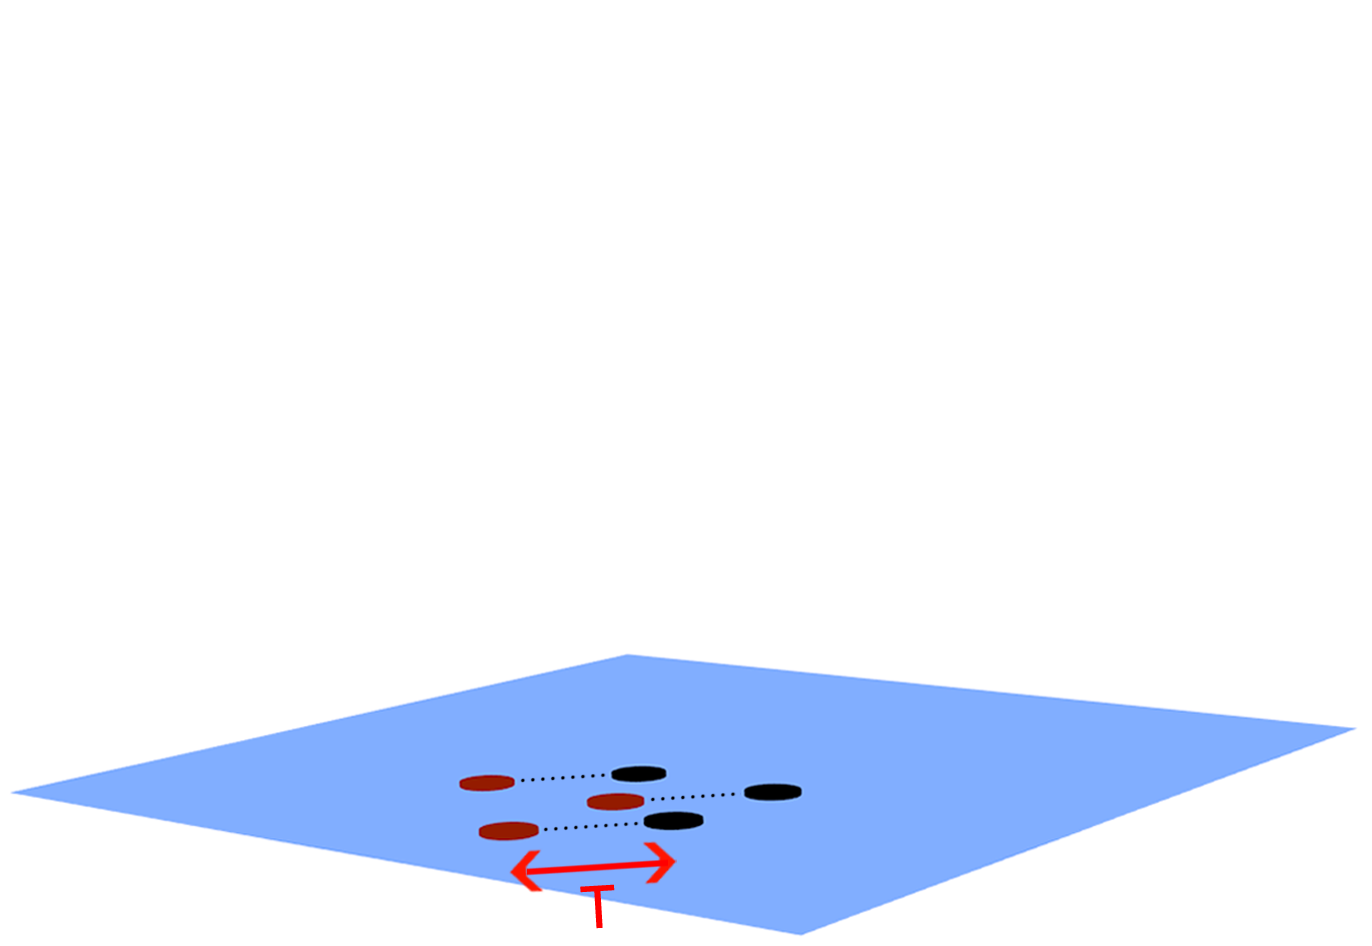
\includegraphics[width=0.33\linewidth]{images/visual_odometry3.png}}
 \end{center}
  \caption{Overview of the visual odometry algorithm. In \ref{visual-slam-visual-odometry1} features from the previous frame $f_{t-1}$ are transformed to corresponding 2D world coordinates using ray-casting. In \ref{visual-slam-visual-odometry2} this step is repeated for the newest frame $f_t$. In both frames the same three features are found, at different locations in the frame. These differences indicate the AR.Drone has moved. Features from this new frame $f_t$ (red circles) are matched against the features from the previous frame (black circles). In \ref{visual-slam-visual-odometry3} a transformation is computed between the world coordinates of both feature sets. This transformation describes the movement $T$ of the AR.Drone between both frames.}
  \label{visual-slam-visual-odometry}
\end{figure}


Each descriptor from frame $f_t$ is matched against the most similar descriptor from the previous frame $f_{t-1}$.
For each match $C(d_t, d_{t-1})$ the 2D world coordinates $(x_{w, d_t}, y_{w, d_t})$ and $(x_{w, d_{t-1}}, y_{w, d_{t-1}})$ of both descriptors are already computed.
These point pairs can be used to calculate a transformation between the points from the last frame and the previous frame.
This transformation describes the movement (e.g., translation) of the AR.Drone between the last two frames.
The transformation is computed using the method described in Section \ref{sec:pose-recovery}.
Now, the velocity is computed using:
\begin{equation}
V_x = Tx / \Delta t
\end{equation}
\begin{equation}
V_y = Ty / \Delta t
\end{equation}
where $V$ is the velocity and $\Delta t$ is the time between the last two frames.



	\section{Elevation mapping using an ultrasound sensor}
	\label{sec:elevation_map}
An elevation map can be used to improve navigation capabilities of both aerial and ground robots.
For example, ground robots can use elevation information to plan routes that avoid obstacles.
As stated in Section \ref{sec:related-research-elevation-mapping}, no publications were found that address the problem of elevation mapping using a single airborne ultrasound sensor.
%At first glance this seems unlikely, because a significant percentage of MAVs is equipped with an ultrasound sensor, commonly used for altitude stabilization.
%However, 
The fundamental limitations of an ultrasound sensor make it hard to build an elevation map.
Two issues are described below.

%\subsection{Fundamental issues}
The first issue is the unknow true altitude $z_{true}$ of the vehicle.
When a MAV is flying above a perfectly flat floor, the measured altitude $z_{sensor}$ is equal to the true altitude $z_{true}$.
However, when an obstacle comes in range of the ultrasound sensor, the measured distance $z_{sensor}$ decreases and is not equal to the true altitude $z_{true}$, meaning that $z_{true}$ cannot be derived from the ultrasound sensor directly.
When the true altitude is unknown, it is impossible to determine the floor's elevation from the distance measurements using the following equation:
\begin{equation}
elevation = z_{true} - z_{sensor}
\end{equation}
%When the MAV is flying above a flat floor without obstacles, the vehicle will remain at a fixed altitude $z$.
%However, when obstacles come in range of the ultrasound sensor, the measured distance $z_{sensor}$ decreases and the vehicle will increase its true %altitude $z_{true}$ by stabilizing the measured altitude $z_{sensor}$.
%Because $z_{sensor} \neq z_{true}$, the true altitude of the vehicle cannot be derived directly from the sensors.
%When the true altitude of the vehicle is unknown, it is hard to use distance measurements to determine the height of obstacles.

Another limitation of using an ultrasound sensor for elevation mapping is the resolution of the sensor.
As described in Section \ref{sec:ultrasound_altimeter}, an ultrasound sensor is unable to obtain precise directional information about objects.
Sound progragates in a cone-like manner.
Due to this property, the sensor acquires entire regions of constant depth instead of discrete depth points.
As a result, the ultrasound sensor can only tell there is an elevation at the measured distance somewhere within the measured cone.
This makes it hard to accurately determine the contours of obstacles.

A third difficulty is related to the altitude stabilization of the AR.Drone (Section \ref{sec:platform-controls}).
The AR.Drone will change its absolute altitude when an altitude difference is detected.
This complicates the detection of elevations, since it cannot be assumed the absolute altitude will remain approximately the same when flying above an object.

The remaining part of this section describes a method to extract elevation information from an airborne ultrasound sensor.
The true altitude of the AR.Drone is modeled as the combination of the measured altitude $z_{sensor}$ and the estimated elevation of the floor $\delta$ below the vehicle:
\begin{equation}
z_{true} = \delta + z_{sensor}
\end{equation}
where the elevation $\delta$ is unknown and needs to be recovered from the ultrasound measurements.

A key part of recovering $\delta$ is a finite-state machine that describes \textit{elevation events}.
A schematic overview of the finite-state machine is given in Figure \ref{fig:elevation_map_fsm}.
This finite-state machine has three different states: \\ $\{ \text{NONE}, \text{UP}, \text{DOWN} \}$.
\begin{comment}
$\left \{ {
\begin{array}{c c c} \text{NONE} & \text{UP} & \text{DOWN} \end{array}
} \right \}$
\end{comment}
State NONE indicates no significant elevation changes are occuring, state UP indicates a significant increase of elevation is detected and state DOWN indicates a significant decrease of elevation is detected.

\begin{figure}[htb]
\centering
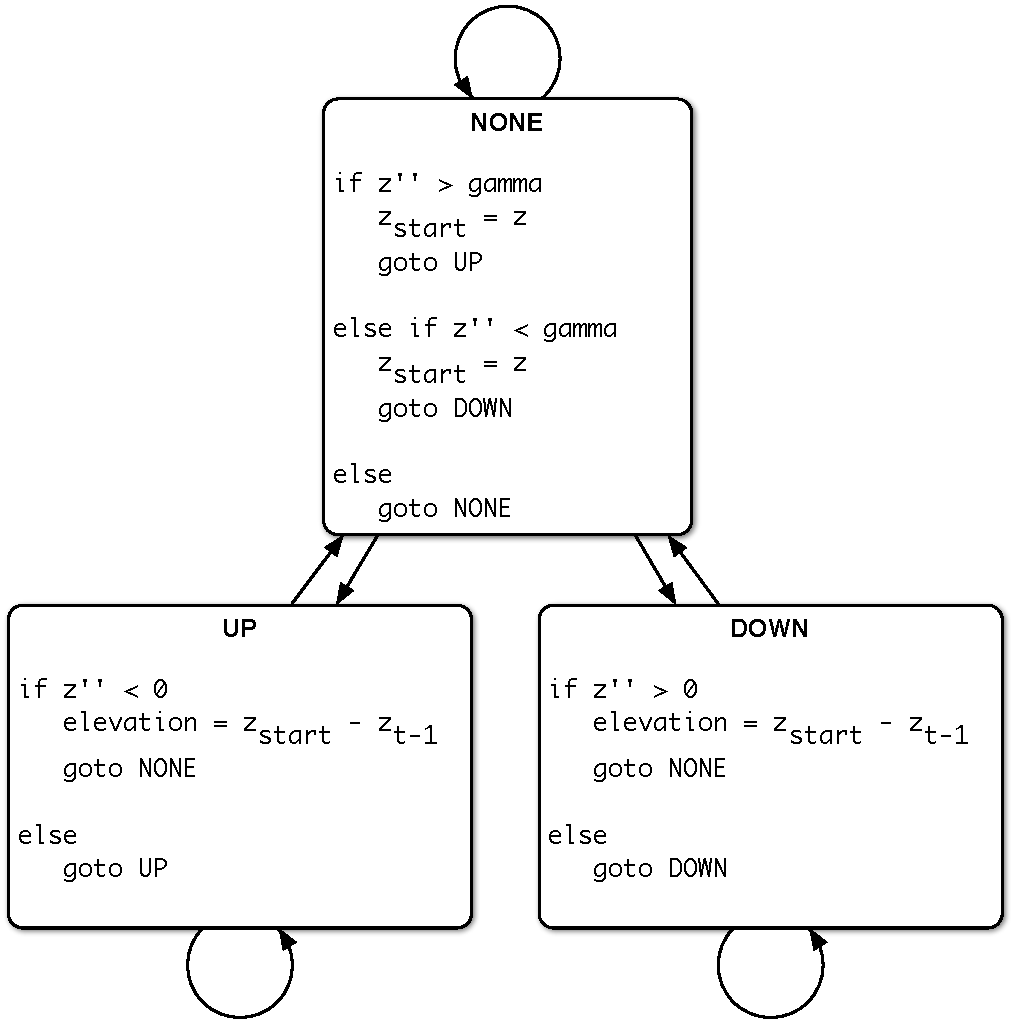
\includegraphics[width=10cm]{images/elevation_map_fsm.pdf}
\caption{Schematic overview of the finite-state machine used for elevation mapping. $z''$ is the second order derivative of the ultrasound distance measurement.}
\label{fig:elevation_map_fsm}
\end{figure}

Elevation changes are detected using a filtered second order derivative (acceleration) of the ultrasound measurement $z_{sensor}$.
Obstacles that enter or leave the range of the ultrasound sensor result in sudden changes in measured ultrasound distance.
These changes are detected when the second order derivative exceeds a certain threshold $\gamma_{elevationEvent}$ and an elevation event is triggered.
The threshold $\gamma_{elevationEvent}$ was carefully chosen such that altitude corrections performed by the AR.Drone altitude stabilization are not detected as being elevation events.
The second order derivative is filtered by adding it to the altitude vector $h^W$ of the EKF state vector.
An elevation event ends when the sign of the second order derivative switches.
This happens when the AR.Drone altitude stabilization starts to change the absolute altitude to compensate for the change in measured altitude.
Now, the elevation change can be recovered by substracting the measured distance at the end of the elevation event from the measured distance before the elevation event was triggered:
\begin{equation}
\Delta\delta_{t} = z_{sensor, t-\Delta t-1} - z_{sensor, t-1}
\end{equation}
where $\Delta\delta_{t}$ is the elevation change during an elevation event, $\Delta t$ is the duration of an event, $z_{sensor, t-\Delta t-1}$ is the distance measurement before the event started and $z_{sensor, t-1}$ is the distance measurement when the event ended.
The total elevation is given by:
\begin{equation}
\delta_{t} = \delta_{t-1} + \Delta\delta_{t}
\end{equation}

\begin{figure}[htb!]
  \begin{center}
    \subfigure[Response]{\label{fig:elevation_method}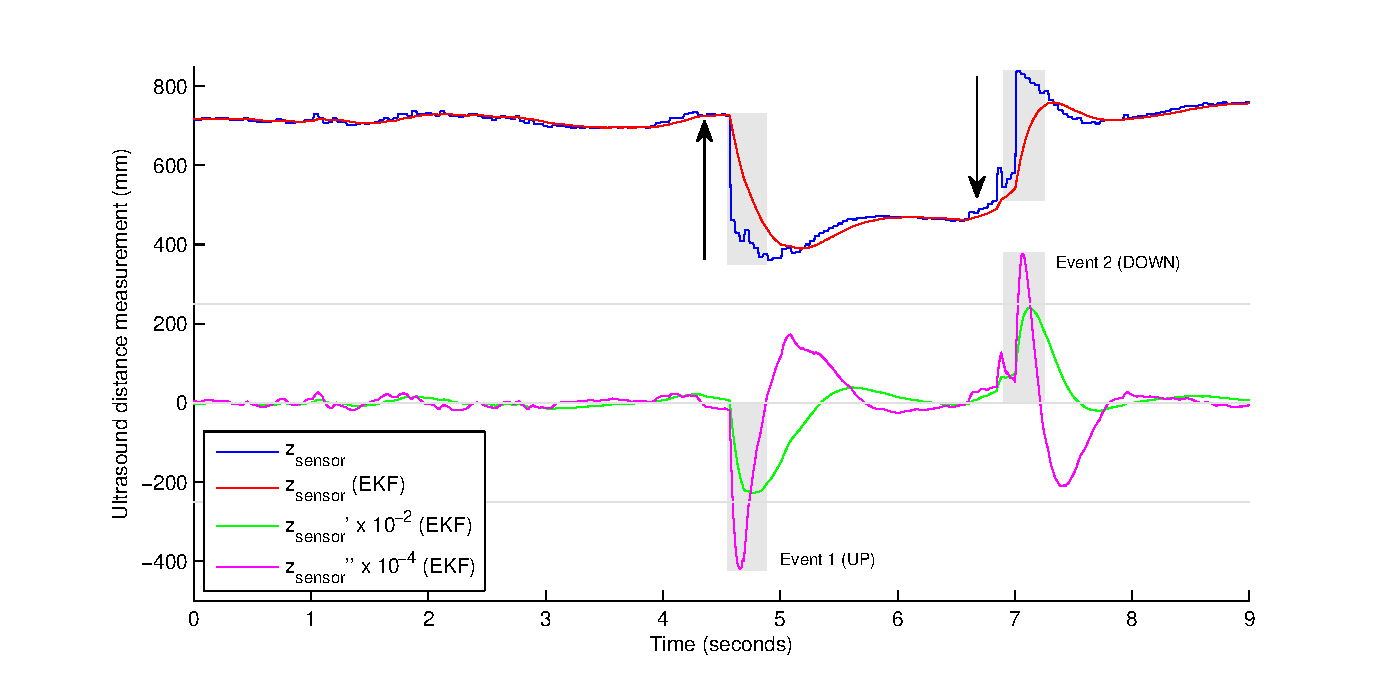
\includegraphics[width=\linewidth]{images/elevation_map.eps}}
    \subfigure[Corresponding elevation]{\label{fig:elevation_method_area}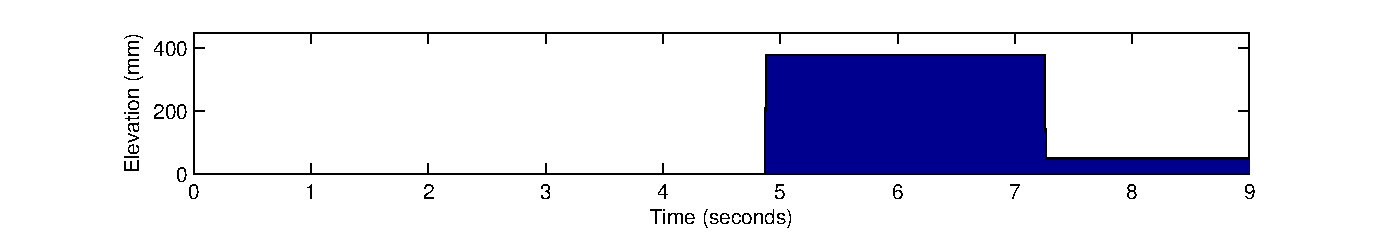
\includegraphics[width=\linewidth]{images/elevation_map_area.eps}}
 \end{center}
\caption{a) Response of the ultrasound sensor when flying over an object of approximately $(60,60,40)\small{mm}$. The lightgray lines indicate the threshold $\gamma_{elevationEvent}$ and null-line. When the second order derivative (magenta line) exceeds the threshold, an event is started (lightgrey rectangle). An event ends when the derivative swaps sign. Each arrow indicates the change in elevation caused by the event. The first event increases the elevation when entering an object and the second event decreases the elevation when leaving the object.
Between both events, the AR.Drone performs an altitude correction, as can be seen by the relatively slow increasement of distance. This increasement is not infomative about the elevation and is ingnored by the elevation mapping method.\\ b) Elevation $\delta$ below the AR.Drone over time. The elevation increases to approximately $40\small{cm}$ when flying above an obstacle. The elevation is decreased when the obstacle is out of the ultrasound sensor's range. There is a small error between both elevation events, resulting in a small false elevation ($\pm 50\small{mm}$) after the AR.Drone flew over the obstacle and is flying above the floor again.}
  \label{visual-slam-elevation-method}
\end{figure}

\begin{comment}
\begin{figure}[htb]
\centering
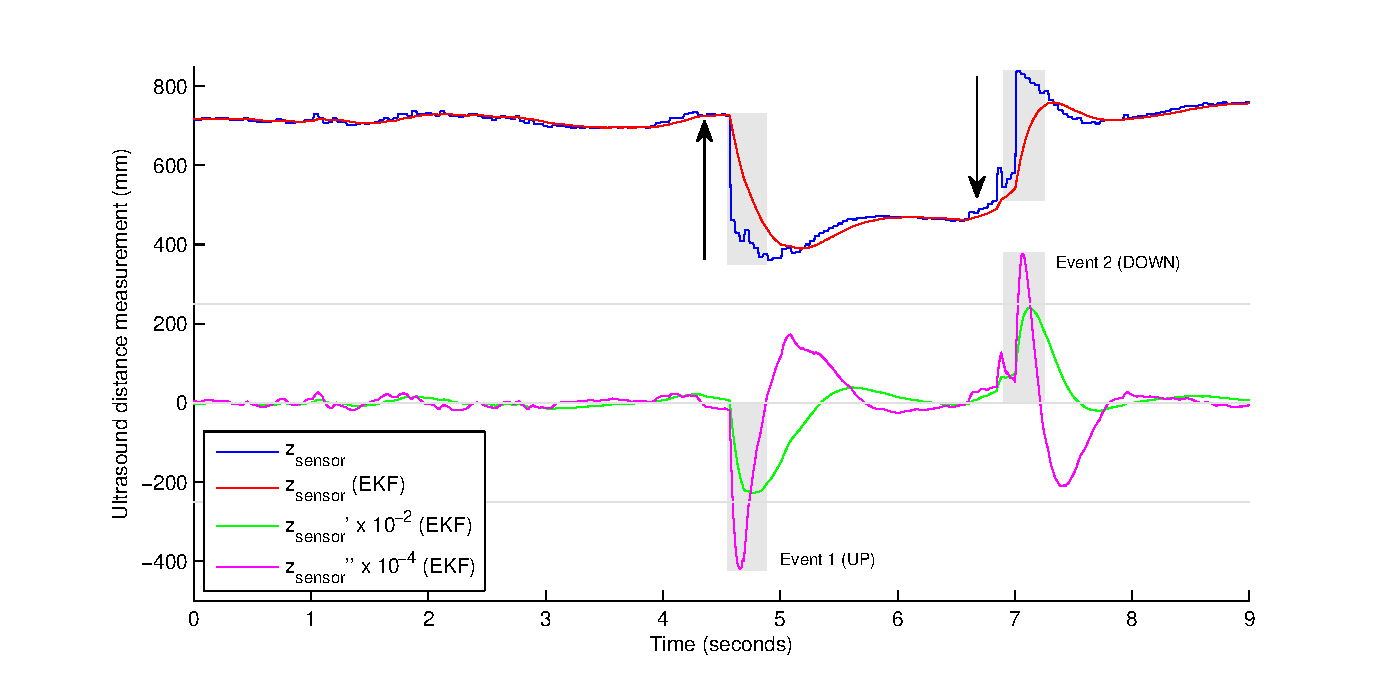
\includegraphics[width=\linewidth]{images/elevation_map.eps}
\caption{Response of the ultrasound sensor when flying over an object of approximately $(60,60,40)\small{mm}$. The lightgray lines indicate the threshold $\gamma_{elevationEvent}$ and null-line. When the second order derivative (magenta line) exceeds the threshold, an event is started (lightgrey rectangle). An event ends when the derivative swaps sign. Each arrow indicates the change in elevation caused by the event. The first event increases the elevation when entering an object and the second event decreases the elevation when leaving the object.
Between both events, the AR.Drone performs an altitude correction, as can be seen by the relatively slow increasement of distance. This increasement is not infomative about the elevation and is ingnored by the elevation mapping method.}
\label{fig:elevation_method}
\end{figure}
\begin{figure}[htb]
\centering
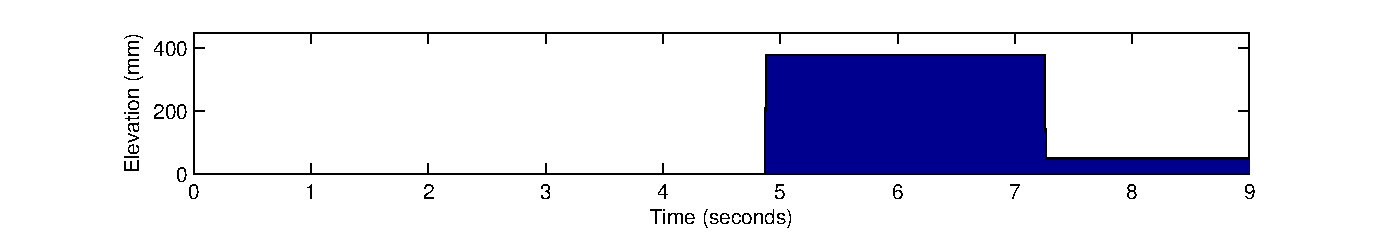
\includegraphics[width=\linewidth]{images/elevation_map_area.eps}
\caption{Elevation $\delta$ below the AR.Drone over time. The elevation increases to approximately $40\small{cm}$ when flying above an obstacle. The elevation is decreased when the obstacle is out of the ultrasound sensor's range. There is a small error between both elevation events, resulting in a small false elevation ($\pm 50\small{mm}$) after the AR.Drone flew over the obstacle and is flying above the floor again.}
\label{fig:elevation_method_area}
\end{figure}
\end{comment}

The elevation information is stored in a grid that is similar to the feature map described in Section \ref{sec:feature_map}.
For each ultrasound distance measurement, elevation $\delta_t$ is computed and stored in the grid cells that corresponds to the world coordinates where a line perpendicular to the AR.Drone body intersects the world plane.
These world coordinates are the position where the center of the ultrasound sensor's cone hits the floor.
Because the exact size of an object is unknown, the elevation is written to all grid cells within a radius $\gamma_{elevationRadius}$ around the intersection point.
This process is visualized in Figure \ref{visual-slam-elevation-map1} and \ref{visual-slam-elevation-map2}.

This approach may lead to cases where the size of an obstacle is overestimated in the elevation map, as can be seen in Figure \ref{visual-slam-elevation-map2}.
Therefore, an additional refinement step is added. %. to the elevation mapping methods.
If no elevation is measured ($\delta_t \approx 0$), it can be assumed there is no obstacle inside the cone of the ultrasound sensor.
Using this assumption, all grid cells within the cone can be resetted to zero elevation and locked to prevent future changes.
This refinement step is visualized Figure \ref{visual-slam-elevation-map3}.
The radius of the cone is computed using the following equation:
\begin{equation}
r = tan (\alpha_{ultrasound} \times z_{sensor})
\end{equation}
where $r$ is the radius of a cone of height $z_{sensor}$ and $\alpha_{ultrasound}$ is the opening angle of the ultrasound sensor.

\begin{figure}[htb!]
  \begin{center}
    \subfigure[Obstacle enters range]{\label{visual-slam-elevation-map1}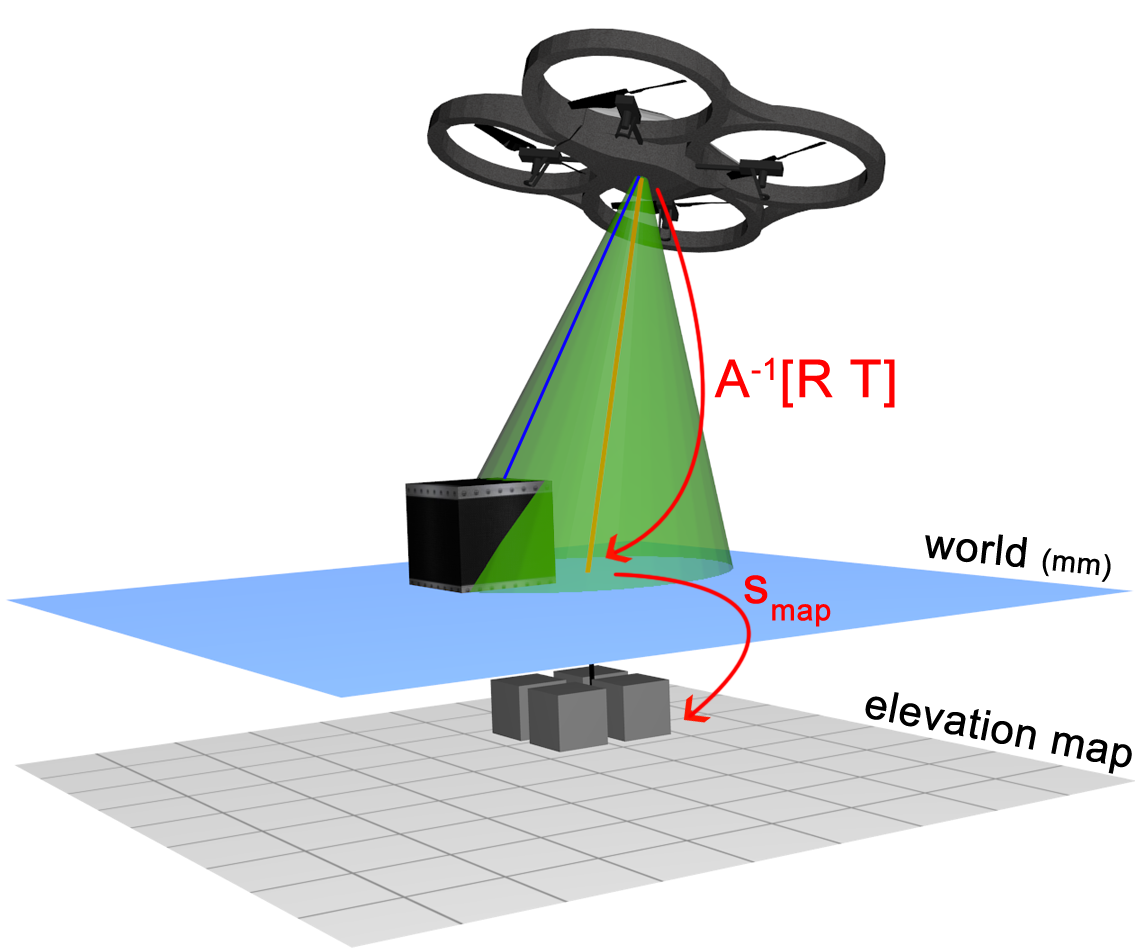
\includegraphics[width=0.33\linewidth]{images/elevation_map1.png}}
    \subfigure[Obstacle in range]{\label{visual-slam-elevation-map2}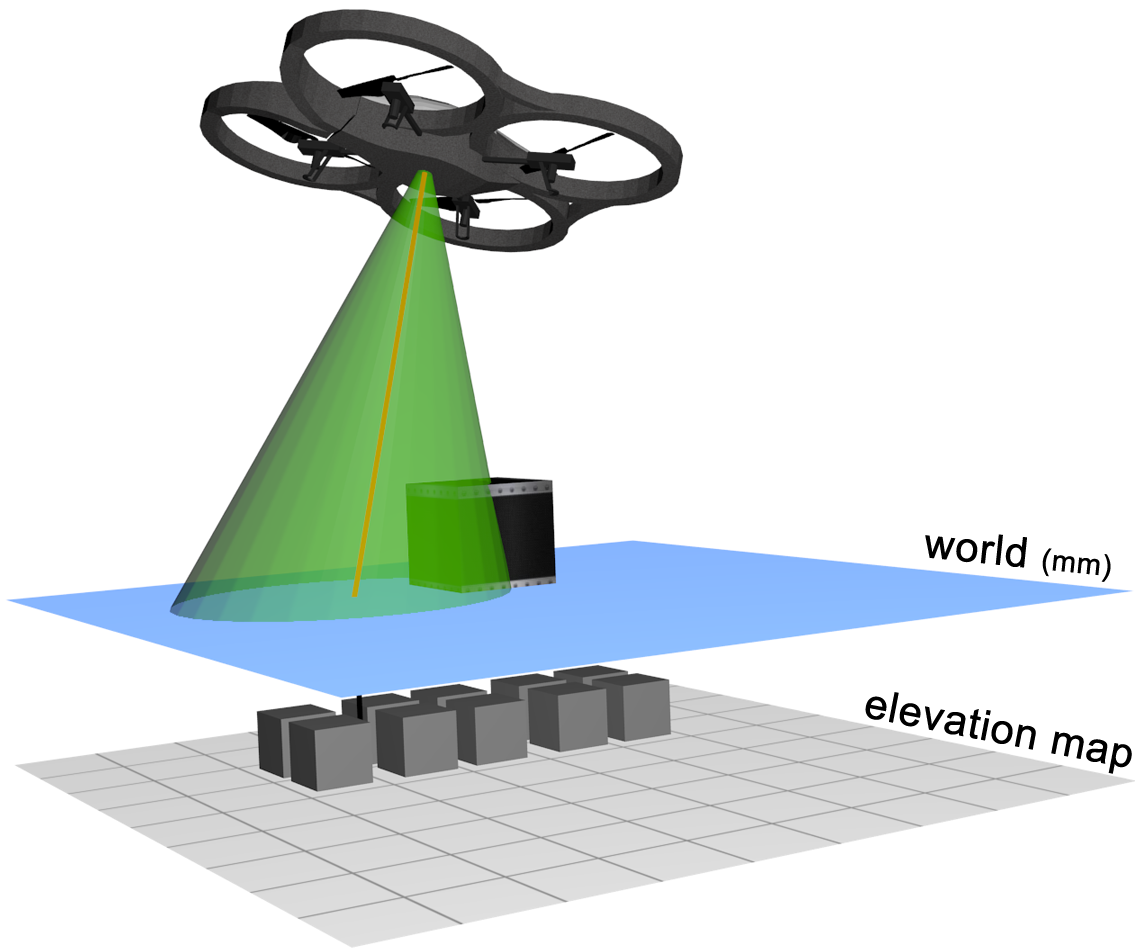
\includegraphics[width=0.33\linewidth]{images/elevation_map2.png}}
    \subfigure[Obstacle out of range]{\label{visual-slam-elevation-map3}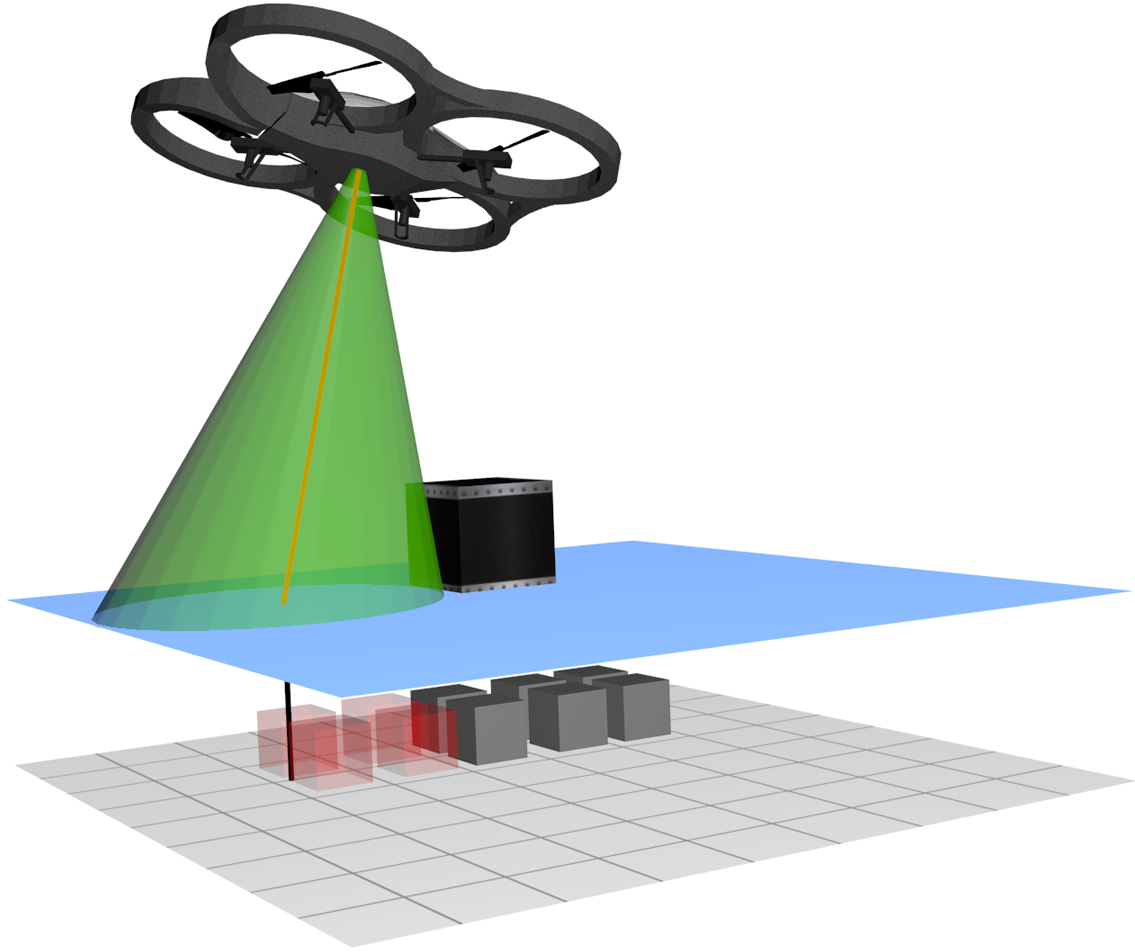
\includegraphics[width=0.33\linewidth]{images/elevation_map3.png}}
 \end{center}
  \caption{Overview of the elevation map updates. The green cone indicates the range of the ultrasound sensor. The red line inside the cone respresents the center of the cone, perpendicular to the AR.Drone's body. In \ref{visual-slam-elevation-map1} and \ref{visual-slam-elevation-map2} an elevation is measured. All grid cells within a radius $\gamma_{elevationRadius}$ around the center of the cone (red line) are updated to store the measured elevation. \ref{visual-slam-elevation-map3} Describes the refinement step. When no elevation is measured, all grid cells within the cone (red cubes) are resetted to zero elevation.}
  \label{visual-slam-elevation-map}
\end{figure}